\begin{comment}
\end{comment}

\chapter{Échantillonnage quasi uniforme et comptage approximatif randomisé}
\label{cha:echantillonnage-quasi-uniforme-comptage-approximatif-randomise}

\begin{comment}
\subsection*{Plan}

\begin{enumerate}
    \item Énoncer brièvement l'algorithme de JVV pour introduire la section
    \item Re-mentionner l'importance du comptage approximatif (en autres en comparaison avec le comptage exact)
    \item Mentionner les concepts nécessaires pour l'algorithme de JVV (auto-réductibilité, échantillonnage quasi aléatoire, comptage approximatif)
\end{enumerate}
\subsection*{Références}
\end{comment}

Les problèmes de décision, ou équivalemment d'existence, et de comptage tel qu'introduits dans le chapitre précédent ne forment qu'une infime partie des problèmes étudiés dans la théorie de la complexité. Ces problèmes se cadrent notamment parmi les problèmes suivants:

\begin{enumerate}[(1)]
    \item \textbf{Existence}: Existe-t-il une solution au problème?
    \item \textbf{Construction}: Construire une solution au problème.
    \item \textbf{Génération uniforme}: Générer uniformément et aléatoirement une solution au problème.
    \item \textbf{Comptage} Combien de solutions satisfont le problème?
\end{enumerate}

Il n'est pas évident de prime abord de comparer la complexité de ces problèmes. Toutefois, dans une publication marquante pour le domaine de la complexité du comptage, Jerrum, Valiant et Vazirani offrent une unique perspective sur l'écart de complexité entre ces différents problèmes~\cite{jerrumRandomGenerationCombinatorial1986}. Les auteurs suggèrent d'abord que la génération uniforme est strictement plus difficile que la construction, et donc que l'existence comme la construction est évidemment au moins aussi difficile que l'existence. De plus, ils avancent que la génération uniforme est plus simple que le comptage, tout en offrant une réduction de la génération uniforme au comptage approximatif. En relaxant le comptage approximatif au comptage approximatif randomisé, ils établissent une correspondance entre ce dernier et la génération quasi uniforme.

Ce travail éclaircit la compréhension de la théorie de la complexité, particulièrement pour la génération uniforme et du comptage. La dernière correspondance entre le comptage approximatif randomisé et la génération quasi uniforme s'avère particulièrement intéressante et forme la base du travail de ce mémoire. Cette inter-réduction mène en effet à un algorithme de comptage approximatif résolvant approximativement certains problèmes de comptage, possédant la propriété d'auto-réductibilité, à l'aide d'un générateur de solutions quasi uniforme. Par souci de commodité, cet algorithme est surnommé \textit{algorithme de JVV} selon le nom de ses auteurs. Parmi ses principaux attraits est sa capacité à obtenir un compte approximatif avec un nombre polynomial d'appels au générateur de solutions, sous la condition que ce dernier soit génère une distribution de solutions suffisamment uniforme. Cette propriété s'avère particulièrement utile pour les problèmes possédant un nombre exponentiel de solutions comme le problème SAT.

Les trois concepts nécessaires à l'algorithme de JVV sont formalisés dans cette section: l'auto-réductibilité à la section~\ref{sec:auto-reductibilite}, l'échantillonnage quasi-uniforme à la section~\ref{sec:echantillonnage-quasi-uniforme} et le comptage approximatif randomisé à la section~\ref{sec:comptage-approximatif-randomise}. Pour conclure, la section~\ref{sec:algorithme-jvv} présente une description en profondeur de l'algorithme de JVV.

%-----------------------------------------------------------------------------%

\section{Auto-réductibilité}
\label{sec:auto-reductibilite}
 
\begin{comment}
\subsection*{Plan}

\begin{enumerate}
    \item Introduire les concepts d'auto-réductibilité
\end{enumerate}

\subsection*{Références}

1. Hemaspaandra, L. A. The Power of Self-Reducibility: Selectivity, Information, and Approximation. Preprint at https://doi.org/10.48550/arXiv.1902.08299 (2019).

\subsection*{Brouillon}

Introduction de "Autoreducibility" par Trakhtenbrot.

Introduction de "Self-reducibility" par Schnorr et Meyer/Paterson.

Survey paper de Balcázar, Selke, Allender.

Explication simple par Hemaspaandra.
\end{comment}

Avant d'introduire le concept d'auto-réductibilité, il est utile de définir une notion supplémentaire. Les problèmes mentionnés dans l'introduction du chapitre sont souvent définis sur des objets mathématiques discrets, comme les formules propositionnelles, les graphes, les permutations, et bien plus. Ces objets se regroupent sous une même ombrelle, nommée \textit{structure combinatoire}, définie comme un système discret fini comportant des éléments et des relations bien définies. Par exemple, une formule propositionnelle, composée de variables booléennes et de contraintes sous forme d'opérateurs booléens, est associée à un ensemble discret de solutions. Conséquemment, le domaine de l'\textit{énumération combinatoire} cherche à déterminer le nombre d'éléments satisfaisant la relation. Pour le problème SAT, cela consiste à trouver le nombre d'assignements satisfaisant la formule propositionnelle. De manière similaire, l'\textit{optimisation combinatoire} tente de trouver la meilleure solution possible au problème.

L'\textit{auto-réductibilité} (« self-reducibility ») est un concept complexe, essentiel à la compréhension du calcul et de la complexité, découlant de l'introduction de la \textit{réduction automatique} (« autoreducibility »)~\cite{trakhtenbrotAutoreducibility1970, selkeAutoreducibilityFriendsMeasuring2006}. Ces concepts sont particulièrement importants dans le contexte de génération aléatoire et du comptage approximatif, mais aussi pour la réduction entre le problème de décision et les problèmes de recherche.

% La \textit{réduction automatique} peut être introduite informellement de la manière suivante:

\begin{subdefinition}{Réduction automatique}{auto-reductibilite}
    Un problème algorithmique est dit \textit{automatiquement réductible} s'il peut être résolu par un algorithme résolvant d'autres instances du même problème, sans que l'algorithme puisse interroger l'instance particulière qu'il cherche à résoudre.
\end{subdefinition}

Les problèmes automatiquement réductibles contiennent de l'information d'appartenance redondante, c'est-à-dire qu'il existe une structure dans l'ensemble de problèmes pouvant être exploitée pour simplifier le calcul d'une instance donnée. Ainsi, un algorithme peut résoudre une instance en utilisant l'information redondante présente dans d'autres instances, évitant ainsi les requêtes directes à l'instance en question. Connaître la solution à une autre problème peut alors simplifier la résolution du problème initial. 

% \textcolor{mydarkred}{\textit{Exemple: Halting problem?}}

Pour discuter de la génération aléatoire et le comptage approximatif, l'\textit{auto-réductibilité descendante}, une forme limitée de la réduction automatique, est une définition plus adéquate. En effet, cette condition est nécessaire à l'application de l'algorithme JVV.

\begin{maindefinition}{Auto-réductibilité descendante}{auto-reductibilite-informel}
    Un problème algorithmique est dit \textit{auto-réductible descendant} s'il peut être résolu grâce à un algorithme résolvant des instances de taille strictement inférieure.
\end{maindefinition}

% \textcolor{mydarkred}{\textit{Quelle est vraiment la différence entre auto-reducibility et self-reducibility?}}

Cette propriété s'éclaircit en prenant le problème SAT comme exemple. L'auto-réductibilité appliquée au problème de satisfaisabilité s'exprime facilement avec la relation suivante~\cite{hemaspaandraPowerSelfReducibilitySelectivity2020}:
\begin{relation}{Auto-réductibilité pour les problèmes SAT}{auto-reductibilite-sat}
    Soit une constante $n \geq 1$ et une formule propositionnelle $\varphi(x_{1}, x_{2}, \dots, x_{n})$ où $x_{i} \in \set{ 0, 1 }$. Alors,
    \begin{equation*}
        \varphi(x_{1}, x_{2}, \dots, x_{n}) = 1 \iff \varphi(x_{1}=0, x_{2}, \dots, x_{n}) = 1 \lor \varphi(x_{1}=1, x_{2}, \dots, x_{n}) = 1
    \end{equation*}
\end{relation}
Cette relation implique que l'ensemble de solutions d'une instance donnée peut être exprimée comme l'ensemble de solutions de deux instances plus petites du problème. Supposons que l'on souhaite résoudre une instance du problème SAT décrit par la formule CNF $\varphi(x_{1}, x_{2}, \dots, x_{n})$. Soit $\varphi_{0} = \varphi(x_{1}=0, \dots, x_{n})$ et $\varphi_{1} = \varphi(x_{1}=1, \dots, x_{n})$ deux sous-instances de l'instance $\varphi$, où la variable $x_{1}$ est remplacée par 0 et 1 respectivement. Ce faisant, la formule $\varphi$ est alors raccourcie, comme certaines clauses sont satisfaites ou du moins réduites. Pour que l'instance $\varphi$ soit satisfaisable, il est nécessaire qu'au moins une des sous-instances $\varphi_{0}$ et $\varphi_{1}$ soit satisfaisable. Dans le cas contraire, l'instance originale $\varphi$ ne peut être satisfaisable car il n'existe pas de solutions peu importe la valeur de $x_{1}$. Ainsi, il suffit de considérer la disjonction des sous-problèmes possibles du problème original pour résoudre ce dernier. Les sous-problèmes obtenus étant aussi des formules propositionnelles, ceux-ci peuvent aussi être décomposés en problème de taille inférieure récursivement. Notons qu'il n'est pas nécessaire de construire la relation~\ref{rel:auto-reductibilite-sat} avec la variable $x_{1}$, n'importe quelle variable $x_{i}$ peut aussi être utilisée. 

% Plus précisément, le problème SAT est décrit comme une auto-réductibilité à longueur décroissante 2-disjonctive. Ici, 2-disjonctive fait référence à une formule propositionnelle dans une disjonction ($\lor$) d'une conjonction ($\land$) d'au plus deux variables. Longueur décroissante, ou descendante, signifie que l'algorithme résout des instances de taille strictement inférieure.

La relation~\ref{rel:auto-reductibilite-sat} exemplifie une deuxième façon de voir l'auto-réductibilité: la résolution partielle d'une instance d'un problème laisse une plus petite instance du même type de problème. Une interprétation alternative est qu'une instance peut être résolue en résolvant des plus petites instances et en assemblant les sous-instances ensemble, tel l'assemblage d'un casse-tête. 

Afin d'obtenir une meilleure perspective sur la notion d'auto-réductibilité, il est pertinent d'exprimer la structure d'une relation auto-réductible $\varphi$ sous la forme d'un arbre orienté, nommé \textit{arbre d'auto-réductibilité}, illustré à la figure~\ref{fig:arbre-auto-reductibilite}. Dans cet arbre, les sommets représentent à la fois une chaîne de bits $w$ de taille $m$ et une instance de problème $\varphi_{w}$, où $\varphi_{w}$ représente la sous-instance du problème $\varphi$ dont les premières variables sont remplacées par la chaîne de bits $w$. Le sous-problème est alors dit \textit{fixé} par le préfixe $w$. Les arrêtes du graphe représentent l'assignement d'une variable. La racine de l'arbre correspond à l'instance du problème initial $\varphi$ ainsi qu'à une solution partielle nulle. Les enfants de cette racine sont par la suite donnés par les sous-instances $\varphi_{w}$ pour tous les préfixes $w$ de taille $1$ possibles. Le reste de l'arbre est défini récursivement de la même manière en augmentant la taille de la chaîne de bits $w$ à chaque niveau jusqu'aux feuilles de l'arbre. Ces feuilles représentent finalement une entrée au problème $\varphi$, étant soit une solution ou une non-solution au problème.

\begin{figure}[h!]
    \centering
    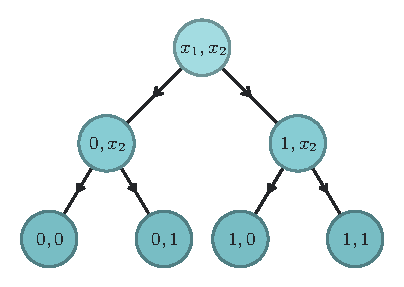
\includegraphics[width=0.6\textwidth]{figures/self-reducibility-tree.pdf}
    \caption[Arbre d'auto-réductibilité]{Un exemple de l'arbre d'auto-réductibilité pour une formule CNF $\varphi(x_{1}, x_{2})$. Les sommets représentent des attributions de littéraux dans $\varphi$ alors que les arêtes orientées indiquent l'affectation d'un littéral.}
    \label{fig:arbre-auto-reductibilite}
\end{figure}

L'auto-réductibilité est simplement généralisable aux problèmes dont les variables peuvent prendre $d$ valeurs, dit auto-réductibilité $d$-disjonctive, en prenant la disjonction sur les $d$ valeurs possibles. Le degré de l'arbre est en conséquence donné par $d$. Notons aussi que l'arbre d'auto-réductibilité est aussi parfois défini tel les feuilles correspondent uniquement à des solutions au problème auto-réductible. Dans ce cas, les non-solutions ne sont pas incluses dans les ramifications de l'arbre.

% \textcolor{mydarkred}{\textit{https://ics.uci.edu/~vazirani/book.pdf}}

% Jusqu'à présent, l’auto-réductibilité a été étudiée principalement dans le cadre du problème SAT. Une vaste étendue de problèmes possèdent toutefois cette propriété, signifiant qu'une généralisation est utile. Ainsi, 

Par complétude, une définition rigoureuse de l'auto-réductibilité dans le sens de Schnorr~\cite{schnorrOptimalAlgorithmsSelfReducible1976} est donnée. Celle-ci permet l'introduction d'un langage pertinent pour le reste de ce chapitre.
\begin{maindefinition}{Auto-réductibilité descendante}{auto-reductibilite-formel}
    Soit $\Sigma^{*}$ un ensemble fixe et fini encodant les instances d'un problème ainsi que leurs solutions. Soit $R \subseteq \Sigma^{*} \times \Sigma^{*}$ une relation binaire assignant à chaque instance de problème $x \in \Sigma^{*}$ un ensemble de solutions $\set{ y \in \Sigma^{*} : xRy }$. Une relation $R \subseteq \Sigma^{*} \times \Sigma^{*}$ est auto-réductible si et seulement si
    \begin{enumerate}[(1)]
        \item il existe une fonction calculable en temps polynomial $g \in \Sigma^{*} \to \mathbb{N}$ tel que $xRy \implies \lvert y \rvert = g(x)$;
        \item il existe une fonction calculable en temps polynomial $\psi \in \Sigma^{*} \times \Sigma^{*} \to \Sigma^{*}$ et $\sigma \in \Sigma^{*} \to \mathbb{N}$ satisfaisant
        \begin{align*}
            & \sigma(x)=O(\log |x|) \\
            & g(x)>0 \Rightarrow \sigma(x)>0 \quad \forall x \in \Sigma^{\star} \\
            & |\psi(x, w)| \leqslant|x| \quad \forall x, w \in \Sigma^{\star}
        \end{align*}
        et tel que, pour tout $x \in \Sigma^{*}, y=y_1 \ldots y_n \in \Sigma^{*}$, 
        \begin{equation*}
            \left\langle x, y_1 \ldots y_n \right\rangle \in R \Leftrightarrow \left\langle \psi \left( x, y_1 \ldots, y_{\sigma(x)} \right), y_{\sigma(x)+1} \ldots y_n \right\rangle \in R
        \end{equation*}
    \end{enumerate}
\end{maindefinition}

Démystifions cette définition. Le problème SAT est un exemple de relation binaire $R$, où $x$ encode une formule booléenne et $y$ encode un assignement satisfaisable parmi l'ensemble des entrées possibles $\Sigma^{*}$ tel que

\begin{equation}
    \begin{aligned}
    R = \{ \braket{x, y} : \ & x \in \Sigma^{*} \text{ encode une formule booléenne } B, \\ 
    & y \in \Sigma^{*} \text{ est un assignement satifaisable de } B \} \,.
    \end{aligned}
\end{equation}

% \textcolor{mydarkred}{\textit{https://era.ed.ac.uk/bitstream/handle/1842/11392/Sinclair1988.pdf?sequence=1}}
% \textcolor{mydarkred}{\textit{$\Sigma$ contre $\Sigma^{*}$}}

La notation $xRy$ signifie que $y$ est une solution valide à l'instance $x$. La première condition implique que la taille des solutions, donnée par la fonction $g$, est bornée par une fonction calculable en temps polynomial. La deuxième condition implique que, pour une instance $x$ et un préfixe $w$ de taille $g(x)$ de n'importe quelle solution $y$ au problème $x$, $\psi$ donne une instance $x'$ dont les solutions sont exactement celles qui, lorsque concaténées avec $w$, forme les solutions de $x$. La fonction $\sigma$ donne alors la granularité des solutions, c'est-à-dire le nombre de caractères de $y$ utilisés pour réduire l'instance $x$. Plus précisément, $\psi(x, w) \leq \lvert x \rvert$ assure que la taille du problème diminue à mesure que la réduction se poursuit. L'implication $g(x) > 0 \implies  \sigma(x) > 0$ signifie que la réduction continue si la taille de l'instance $x$ est non-nulle. La dernière relation énonce que la résolution du problème pour $\braket{x, y}$ peut être réduite à la résolution d'instances de taille inférieure, c'est-à-dire que $\braket{x, y_{1}\dots y_{n}}$ est reliée à $\braket{\psi(x, y_{1}\dots y_{n}), y_{\sigma(x)+1}\dots y_{n}}$.

Tous les problèmes \textsf{NP}-complet sont auto-réductibles~\cite{goldreichComputationalComplexityConceptual2008}, mais ce n'est pas le cas pour tous les problèmes de la classe \textsf{NP}~\cite{khullerPlanarGraphColoring1991a}. De nombreux problèmes \textsf{NP} sont aussi auto-réductible descendant. Ces observations impliquent que l'algorithme de JVV s'applique en théorie à de nombreux problèmes intéressants. Toutefois, trouver une relation auto-réductible en pratique n'est pas toujours évident.

La définition de l'auto-réductibilité utilisée dans cette section s'applique principalement à l'équivalence entre l'échantillonnage quasi uniforme et le comptage approximatif randomisé. Cependant, une définition alternative~\cite{goldreichComputationalComplexityConceptual2008} est souvent introduite pour l'équivalence entre les problèmes de décision et les problèmes de recherche, où un problème de recherche ne demande pas de montrer l'existence d'une solution, mais de construire une telle solution. En effet, si un problème est auto-réductible à ce sens, alors le problème de recherche est de la même complexité que le problème de décision. 

% \textcolor{mydarkred}{\textit{la definition est due a qui?}}

%-----------------------------------------------------------------------------%

\section{Échantillonnage quasi uniforme}
\label{sec:echantillonnage-quasi-uniforme}

\begin{comment}
\subsection*{Plan}

\begin{enumerate}
    \item Introduire les FPAUS
    \item Introduire la distance en variation totale et la non-uniformité
\end{enumerate}

\subsection*{Références}
\end{comment}

L'\textit{échantillonnage uniforme} de structures combinatoires consiste à générer aléatoirement des solutions de manière uniforme, c'est-à-dire avec une probabilité suivant la distribution de probabilité uniforme des solutions, à un problème donné. Le problème de génération uniforme est assez méconnu, mais possède plusieurs applications dont la construction d'éléments représentatifs d'un ensemble, la formulation de conjectures pour un ensemble ou la vérification fonctionnelle du matériel informatique~\cite{jerrumFastUniformGeneration1990, chakrabortyScalableNearlyUniform2013}.

La génération uniforme étant une demande plutôt rigide, il est parfois nécessaire de relaxer la condition d'uniformité pour une quasi-uniformité. Une distribution quasi uniforme est en pratique indiscernable d'une distribution uniforme, mais ce relâchement facilite certaines preuves. La \textit{distance en variation totale} est une mesure de distance statistique définie entre deux distributions de probabilité, déterminant la similitude entre ces distributions. Cette mesure permet entre autres de caractériser à quel point une distribution quasi uniforme se rapproche de la distribution uniforme.

\begin{subdefinition}{Distance en variation totale}{tvd}
    Soit deux distributions de probabilité $P$ et $Q$ définies sur un ensemble dénombrable $\chi$. La distance en variation totale est
    \begin{equation*}
        \lVert P - Q \rVert_{TV} \equiv \frac{1}{2} \sum_{x \in \chi} \lvert P(x) - Q(x) \rvert \,. 
    \end{equation*}
\end{subdefinition}

Une distribution est alors dite quasi uniforme si sa distance en variation totale avec la distribution uniforme est suffisamment petite. Une définition commune demande que cette distance diminue proportionnellement avec l'inverse de la taille du problème. Un \textit{échantillonneur quasi uniforme de tolérance $\xi$} génère alors des solutions selon une distribution de probabilités où la distance en variation totale entre celle-ci et la distribution uniforme est plus petite que $\xi$~\cite{jerrumCountingSamplingIntegrating2003}.

\begin{maindefinition}{Échantillonneur quasi uniforme}{fpaus}
    Un échantillonneur quasi uniforme pour un ensemble de solutions $S \subseteq \Sigma^{*} \times \Sigma^{*}$, où $S$ représente la relation entre les instances d'un problème $x$ et de ses solutions $y \in  S(x)$, est un algorithme aléatoire prenant en entrée une instance $x \in \Sigma^{*}$ et une tolérance d'échantillonnage $\xi > 0$ et qui génère une solution $y \in S(x)$ tel que
    \begin{equation*}
        \lVert Y - U \rVert_{TV} \leq \xi
    \end{equation*}
    où $Y$ est la distribution de probabilité de $y$ et $U$ est la distribution de probabilité uniforme sur $S(x)$. Si l'algorithme s'exécute en temps borné par un polynomial en $\lvert x \rvert$ et en $\ln (\xi^{-1})$, on parle d'échantillonneur quasi uniforme pleinement polynomial (« Fully Polynomial Almost Uniform Sampler») (FPAUS).
\end{maindefinition}

 Une notion supplémentaire est introduite dans ce mémoire afin de simplifier la notation. La \textit{non-uniformité}, de manière similaire à la distance en variation totale, décrit la distance entre une distribution de probabilité $Q$ et la distribution de probabilité uniforme $U$.

\begin{maindefinition}{Non-uniformité}{non-uniformite}
    Soit la distribution de probabilité $P$ et la distribution de probabilité uniforme $U$ tel que $U(x) = 1/\lvert x \rvert$ définies sur un ensemble dénombrable $\chi$. La non-uniformité est
    \begin{equation*}
        \eta \equiv \frac{1}{2} \sum_{x \in \chi} \lvert P(x) - U(x) \rvert \,. 
    \end{equation*}
\end{maindefinition}

Un échantillonneur quasi uniforme de tolérance $\xi$ possède en conséquence une non-uniformité plus petite que $\xi$.

%-----------------------------------------------------------------------------%

\section{Comptage approximatif randomisé}
\label{sec:comptage-approximatif-randomise}

\begin{comment}
\subsection*{Plan}

\begin{enumerate}
    \item Introduire les FPRAS
    \item Introduire les algorithmes de comptage classique connus (ex.: Stockmeyer et JVV)
\end{enumerate}

\subsection*{Références}

1. Stockmeyer, L. The complexity of approximate counting. in Proceedings of the fifteenth annual ACM symposium on Theory of computing 118–126 (Association for Computing Machinery, New York, NY, USA, 1983). doi:10.1145/800061.808740.
\end{comment}

Comme mentionné au chapitre~\ref{cha:complexite-du-denombrement}, les problèmes de comptage sont d'une grande complexité et nécessitent en pratique des méthodes approximatives pour la résolution de problèmes de grandes tailles. Le \textit{comptage approximatif randomisé} simplifie davantage les attentes en ne demandant une solution approximative valide qu'avec une certaine probabilité. Un \textit{schéma d'approximation randomisé de tolérance $\varepsilon$} se définit de manière similaire à l'algorithme d'approximation pour l'optimisation décrit à la section~\ref{sec:intractabilite-approximation-et-optimisation}. 

\begin{maindefinition}{Schéma d'approximation randomisé}{fpras}
    Un schéma d'approximation randomisé pour un problème de comptage $f: \Sigma^{*} \to \mathbb{N}$ est un algorithme randomisé prenant en entrée une instance d'un problème $x \in \Sigma^{*}$ et une tolérance d'erreur $\varepsilon > 0$ et qui génère un nombre $N \in \mathbb{N}$ tel que, pour toute instance $x$,
    \begin{equation*}
        \mathrm{ Pr }\left[(1+\varepsilon)^{-1} f(x) \leq N \leq (1+\varepsilon)f(x)\right] \geq \frac{3}{4} .
    \end{equation*}
    Si l'algorithme s'exécute en temps borné par un polynomial en $\lvert x \rvert$ et $\varepsilon^{-1}$, alors on parle de schéma d'approximation randomisé pleinement polynomial (« Fully Polynomial Randomized Approximation Scheme ») (FPRAS).
\end{maindefinition}

La valeur $3/4$ est un nombre arbitraire pouvant être remplacée par n'importe quel nombre dans l'intervalle ouvert $(\frac{1}{2}, 1)$. Ce nombre, représentant la confiance de succès du schéma, peut être augmenté à n'importe quelle valeur $1-\delta$ pour $\delta > 0$ au coût d'un facteur multiplicatif $O(\log(\delta^{-1}))$. Pour ce faire, il suffit de répéter le schéma original $O(\log(\delta^{-1}))$ fois et de prendre la médiane des résultats obtenus.   

%-----------------------------------------------------------------------------%

\section{Algorithme de Jerrum-Valiant-Vazirani}
\label{sec:algorithme-jvv}

\begin{comment}
\subsection*{Plan}

\begin{enumerate}
    \item Introduire le but de l'algorithme de JVV
    \item Vulgariser l'algorithme de JVV
    \item Introduire rigoureusement l'algorithme de JVV
    \item Rajouter l'algorithme complet sous forme de pseudo-code.
\end{enumerate}

\subsection*{Références}

1. Jerrum, M. R., Valiant, L. G. and Vazirani, V. V. Random generation of combinatorial structures from a uniform distribution. Theoretical Computer Science 43, 169–188 (1986).
2. Huber, M. Exact sampling and approximate counting techniques. in Proceedings of the thirtieth annual ACM symposium on Theory of computing 31–40 (Association for Computing Machinery, New York, NY, USA, 1998). doi:10.1145/276698.276709.
\end{comment}


Le travail de Jerrum, Valiant et Vazirani~\cite{jerrumRandomGenerationCombinatorial1986} (voir aussi~\cite{broderHowHardIt1986, sinclairAlgorithmsRandomGeneration1993}) établit une correspondance entre l'échantillonnage quasi uniforme et le comptage approximatif randomisé. Pour ce faire, deux algorithmes permettant le passage d'un problème à l'autre sont présentés. Bien la réduction du comptage à l'échantillonnage est intéressante, elle ne sera discuté que brièvement à la fin de la section comme la réduction d'importance est ici son inverse. L'algorithme de comptage approximatif randomisé, surnommé \textit{algorithme de JVV}, permet de trouver le nombre de solutions d'un problème auto-réductible de la classe \textsf{\#P} à une erreur multiplicative près avec un nombre polynomial d'appels à un générateur de solution quasi uniforme. Le comptage approximatif randomisé est utilisé plutôt que le comptage approximatif en raison de l'impossibilité d'obtenir un résultat déterministe à partir d'une procédure aléatoire.

% \textcolor{mydarkred}{\textit{Expliquer le lien entre les deux concepts et les preuves.}}

\begin{maintheorem}{Algorithme de JVV}{algorithme-jvv}
    Si un problème algorithmique auto-réductible dans \textsf{\#P} de taille $n$ admet un générateur de solutions avec une non-uniformité $\eta = O(1 / n)$, alors le nombre de solutions peut être approximé à une erreur multiplicative $O(\eta n)$ avec une haute probabilité en utilisant un nombre polynomial d'appels au générateur.
\end{maintheorem}

Plus précisément, en exigeant un échantillonneur quasi uniforme pleinement polynomial (FPAUS), l'algorithme de JVV fournit un schéma d'approximation randomisé pleinement polynomial (FPRAS) pour le comptage approximatif de relations auto-réductibles. Plus précisément, pour un problème de $n$ variables, $O(\frac{n^{2} \log \delta^{-1}}{\varepsilon^{2}})$ échantillons sont nécessaires pour obtenir un compte approximatif de tolérance $\varepsilon$ et de confiance $\delta$.

Comment est-ce que l'algorithme de JVV opère? Commençons par introduire l'idée principale derrière l'algorithme pour ensuite donner un exemple simple et compléter avec une description plus formelle. 

Pour mieux comprendre son exécution, l'arbre d'auto-réductibilité, présenté à la section~\ref{sec:auto-reductibilite}, est employé. L'algorithme de JVV implique de se déplacer vers le haut ou vers le bas de cet arbre, en s'intéressant à toutes les sous-instances en chemin. Supposons qu'il est possible d'échantillonner uniformément les solutions de n'importe quelle instance du problème SAT (la généralisation à un échantillonneur quasi uniforme est effectuée plus bas). Commençons d'abord par échantillonner des solutions au problème initial $\varphi$ représenté par la racine de l'arbre. Soit $P_{0}$ et $P_{1}$ les probabilités que la première variable $x_{1}$ soit respectivement de 0 et 1 pour les solutions échantillonnées. Ces probabilités reflètent la proportion de solutions dans chaque sous-arbre. Par la suite, descendons l'arbre vers l'enfant le plus probable $\varphi_{w_{1}}$, représentant la formule $\varphi$ réduite par le préfixe $w_{1}$, en gardant en mémoire la probabilité $P_{w_{1}}$. Comme l'échantillonneur peut aussi résoudre le problème subséquent, nous pouvons encore déterminer la valeur la plus probable de la variable suivante $x_{2}$ à partir de la probabilité $P_{w_{2}}$. Le processus est répété jusqu'à atteindre les feuilles de l'arbre, en sauvegardant les probabilités $P_{w_{i}}$ le long du chemin $w$ choisi. Au dernier noeud avant les feuilles, nous obtenons une solution avec une probabilité $P_{w_{n}}$. Comme nous sommes à la base de l'arbre, cette probabilité indique le nombre de solutions que possède la dernière sous-instance. En effet, ce sous-arbre contient nécessairement $\frac{1}{P_{w_{n}}}$ solutions, car il y a nécessairement une ou deux solutions à la dernière sous-instance. En remontant l'arbre, on remarque que la sous-instance précédente contient $\frac{1}{P_{w_{n-1}}}$ fois plus de solutions. Par conséquent, le nombre de solutions dans cette partie de l'arbre est de $\frac{1}{P_{w_{n}}} \cdot \frac{1}{P_{w_{n-1}}}$. Continuant cette procédure jusqu'à la racine, nous trouvons que le nombre de solutions est donné par 

\begin{equation}
    N = \frac{1}{P_{w_{0}}} \cdot \frac{1}{P_{w_{m}}} \dots \frac{1}{P_{w_{n}}} = \frac{N}{N_{w_{0}}} \cdot \frac{N_{w_{0}}}{N_{w_{1}}} \dots \frac{N_{w_{n-1}}}{N_{w_{n}}} \,,
\end{equation}

où $N_{w_{i}}$ est le nombre de solutions au problème $\varphi_{w_{i}}$. Éclaircissons maintenant cette idée à l'aide d'un exemple simple illustré à la figure~\ref{fig:algorithme-jvv}. Soit une instance du problème SAT décrite par la formule CNF $\varphi(x_{1}, x_{2}) = \neg x_{1} \land x_{2}$, dont les solutions sont les couples $(0,0)$, $(0,1)$ et $(1,1)$. Un arbre est construit de manière à représenter toutes les sous-instances de l'instance originale. Chaque niveau de l'arbre correspond à l'attribution d'une valeur, 0 ou 1, à une variable, constituant ainsi une sous-instance du problème initial. La racine de l'arbre représente le problème initial et ses deux variables $x_{1}$ et $x_{2}$. La première couche représente les sous-problèmes $\varphi_{0}$ et $\varphi_{1}$ où la première variable est remplacée par 0 et 1 respectivement. Les feuilles représentent les assignations possibles au problème $\varphi$, c'est-à-dire lorsque toutes les variables sont fixées à une certaine valeur. Les arrêtes de l'arbre partant des noeuds du niveau $i$ au niveau $i+1$ décrivent la probabilité qu'une solution au problème commence avec le préfixe $w_{i}$. Maintenant que l'arbre d'auto-réductibilité est construit, comptons le nombre de solutions à la formule $\varphi(x_{1}, x_{2})$. En échantillonnant l'instance originale, nous trouvons que les échantillons possèdent une probabilité $P_{0}=\frac{2}{3}$ de commencer avec la variable $x_{1} = 0$. La sous-instance $\varphi_{0} = \varphi(0, x_{1})$ est donc choisi, comme il s'agit de l'enfant le plus probable, et de nouvelles solutions sont générées. Nous remarquons que celles-ci possèdent la même probabilité $P_{w}=\frac{1}{2}$ de commencer par le préfixe $w=00$ que $w=01$. Après avoir choisi le préfixe $w=01$, le compte est obtenu de la façon suivante $N = (P_{0} \cdot P_{01})^{-1} = 3$.

\begin{figure}[h]
    \centering
    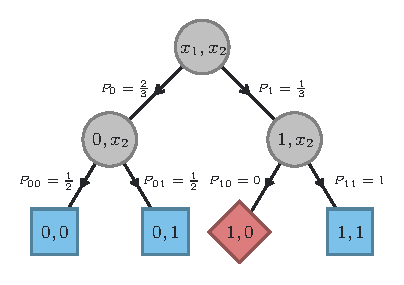
\includegraphics[width=0.55\textwidth]{figures/jvv-algorithm.pdf}
    \caption[Algorithme de Jerrum-Valiant-Vazirani]{Un exemple de l'arbre d'auto-réductibilité dans l'algorithme JVV pour une formule CNF $\varphi(x_{1}, x_{2})$. Les sommets représentent des attributions de littéraux dans $\varphi$, avec les solutions représentées par des carrés bleus et les non-solutions par des losanges rouges. Les arêtes orientées indiquent l'affectation d'un littéral ainsi que sa probabilité associée. En suivant le chemin des probabilités maximales, illustré par une ligne pleine, le comptage est obtenu comme $N = (P_{0} \cdot P_{01})^{-1} = 3$.}
    \label{fig:algorithme-jvv}
\end{figure}

Quelques notes sont ici nécessaires. Le chemin des probabilités maximales est choisi comme une meilleure précision est atteinte avec un plus grand nombre de solutions. De plus, ce choix évite d'obtenir une probabilité nulle, c'est-à-dire lorsque le sous-arbre ne possède aucune solution. Jusqu'à maintenant, le générateur a été considéré comme uniforme. Il est cependant possible d'utiliser une distribution quasi uniforme, qui introduit une petite erreur additionnelle pouvant être absorbée dans la tolérance $\varepsilon$.

Supposons que le nombre exact de solutions pour une instance de problème SAT de $n$ est de $N$. Notons $x_{:m}$ le préfixe de taille $m$ de la chaîne de bits $x$ et $N_{x_{:m}}$ le nombre de solutions commençant avec le préfixe $x_{:m}$. Par la suite, supposons que nous avons accès à un générateur qui échantillonne l'ensemble de solutions uniformément et aléatoirement, tel que chaque solution est échantillonnée avec une probabilité $p^{\star} = \frac{1}{N}$. Pour n'importe quelle solution $z$, on écrit

\begin{align}
    p^\star = \frac1N =&{\ } \frac{N_{z_{:1}}}{N} \cdot \frac{N_{z_{:2}}}{N_{z_{:1}}} \cdots \frac{N_{z_{:n}}}{N_{z_{:n-1}}} \\
    =&{\ } p(z_{:1}) \cdot p(z_{:2}|z_{:1}) \cdots p(z_{:n}|z_{:n-1}) \\
    =&{\ } p(z_{:1}) \prod_{i=1}^{n-1} p(z_{:i+1}|z_{:i}) \,,
\end{align}

où $N_{z_{:n}} \equiv 1$. La probabilité conditionnelle $p(z_{:i+1}|z_{:i}) \equiv N_{z_{:i+1}} / N_{z_{:i}}$ est la probabilité qu'une solution échantillonnée $z'$ soit $z'_{i+1} = z_{i+1}$ sachant que $z'_{:i} = z_{:i}$.  

L'algorithme de JVV pour le comptage approximatif retourne une approximation à un facteur multiplicatif près de $p^{\star}$, et donc de $N$, en approximant les probabilités conditionnelles $p(z_{:i+1}|z_{:i})$. Cela est fait en générant un ensemble d'échantillons $S$ et en approximant les probabilités conditionnelles avec

\begin{equation}
    \tilde p(z_{:i+1}|z_{:i}) = \frac{ \tilde N_{z_{:i+1}} }{ \tilde N_{z_{:i}} } \,,
\end{equation}

où $\tilde{N}_{z_{:i}}$ est le nombre de solutions dans l'ensemble d'échantillons commençant par $z_{:i}$. Donc,

\begin{equation}
    \tilde p^\star = \tilde p(z_{:1}) \prod_{i=1}^{n-1} \tilde p(z_{:i+1}|z_{:i}) \approx \frac1N \,.
\end{equation}

% Les solutions à ce problème sont facilement vérifiable par examination. Le problème SAT étant auto-réductible, un arbre d'auto-réductibilité peut être construit de manière à représenter tous ses sous-problèmes tel qu'illustré à la figure~\ref{fig:algorithme-jvv}. Supposons qu'il soit possible d'estimer 

% Comme décrit à la section~\ref{sec:auto-reductibilite}, chaque noeud de l'arbre est associé une chaîne de bits $w$ de taille $m$ fixant les $m$ premières variables de la formule $\varphi$ ainsi qu'une formule partielle $\varphi_{w}$. 

Le nombre approximatif de solutions est ainsi obtenu. L'algorithme se résume par l'algorithme~\ref{sec:algorithme-jvv}.

\begin{algorithm}[h!]
    \caption{Algorithme de JVV}\label{alg:algorithme-jvv}
    \begin{algorithmic}[1]
    \REQUIRE Formule CNF: $f(n, m)$, Nombre d'échantillons: $n_{s}$

    \STATE $\tilde{N} \leftarrow 1$
    \FOR{$i \in \{1, \dots, n\}$}
    \STATE $S \leftarrow \{ \ \}$
    \WHILE{$\abs{S} < n_{s}$}
    \STATE $m \leftarrow \text{Échantillonnage}(f(n,m))$
    \STATE $S \leftarrow S \cup \set{m}$
    \ENDWHILE
    \STATE $w, \tilde{p} \leftarrow \arg \max_{w' \in \set{ w + 0, w + 1 }} \lvert \set{ s \in S : s_{:\lvert w' \rvert } = w' } \rvert / \lvert S \rvert$
    \STATE $\tilde{N} \leftarrow \tilde{N} / \tilde{p}$
    \ENDFOR
    
    \RETURN $\tilde{N}$
\end{algorithmic}
\end{algorithm}

Finalement, un générateur de solutions aléatoire uniforme peut aussi être construit à partir d'un compteur approximatif en inversant la procédure présentée ci-haut. Pour ce faire, descendons l'arbre d'auto-réductibilité d'un problème $\varphi$ avec $N$ solutions à nouveau. À chaque noeud de l'arbre, comptons approximativement le nombre de solutions au sous-problème $\varphi_{w_{i}}$ et empruntons la prochaine branche avec une probabilité proportionnelle au nombre de solutions dans le sous-arbre, c'est-à-dire $\frac{N_{w_{i+1}}}{N_{w}}$. En suivant cette procédure jusqu'aux racines, une solution sera obtenue avec une probabilité $\frac{1}{N}$.